% write your paper in here

\chapter{Introduction}

\textit{This introduction is a review of genomes assemblies of non-vertebrate animals in preparation with Ramon E. Rivera-Vicéns, Romain Koszul and Jean-François Flot.} \\

The field of genomics is presently thriving, with new genomes of all kind of organisms becoming available every day. For Animalia (i.e. metazoans), efforts have unsurprisingly focused on human's closest relatives (i.e., vertebrates) so far \cite{rice2019}: out of 5,994 metazoan assemblies available in the NCBI database (accessed on April 21rst, 2021) \cite{ncbi}, $\sim$ 67.5\% (3,809) belong to the subphylum Vertebrata. However, from the currently $\sim$2.1 million described metazoan species, only $\sim$73,000 (3.5\%) belong to vertebrates \cite{red_list}. The remaining metazoan phyla, hereafter called "non-vertebrate animals", are thus underinvestigated and lack genetic resources. \\ 

Non-vertebrate animals are found in nearly all known terrestrial and aquatic ecosystems (both marine and freshwater), and represent the diverse branches of the metazoan tree of life (among which vertebrates are just a twig that originated about 600 millions years ago \cite{timetree}). Characterizing the genome structure and gene content of non-vertebrate animals is therefore pivotal for expanding our knowledge regarding the evolution, ecology and biodiversity of metazoans. \\

In recent years, important sequencing efforts have started to tackle the dearth of genomic data for non-vertebrate animals, with a strong focus on arthropods (1,279 assemblies on NCBI). The phylum Arthropoda is very diverse: it consists of more than 1.3 million species, the majority of which belong to the class Insecta ($\sim$1 million species) \cite{Zhang2013}. Insects have a significant impact on agriculture (e.g. as crop pests) and on the transmission of diseases (e.g. malaria and dengue) \cite{li2019}. They also play important beneficial and regulatory roles in natural ecosystems, through pollination and decomposition of organic matter \cite{noriega2018}. Genome sequencing yields invaluable insights into species that are key in the aforementioned processes. For example, various genome projects have targeted insects such as \textit{Bemisia tabaci}, a common crop pest \cite{chen2016}, and the mosquitoes \textit{Aedes aegypti} (vector of yellow fever, dengue and chikungunya) \cite{aedes_aegypti3} and \textit{Anopheles darlingi} (vector of malaria) \cite{marinotti2013}. These studies unveiled, among other findings, expansions of genes involved in insecticide resistance. The genomes of these species are so important for human health and food security that many have actually been sequenced multiple times, either because of the availability of newer sequencing methods or to compare different strains (for instance, three versions of the genome of \textit{Aedes aegypti} \cite{aedes_aegypti, 3d-dna, aedes_aegypti3} were successively published). Many phyla with less direct human implications, however, do not even have a single good-quality genome assembly available to date (e.g., chaetognaths). \\ 

Many other non-vertebrates (and their symbionts) have also shown tremendous importance and relevance with respect to socio-economic impact. Snails, sponges and corals all produce metabolites with biological activities such as anticancer, anti-inflammatory, antibacterial, among others \cite{carroll2021, khalifa2019, ng2015}. Terpenoid metabolites have been found in more than 70 gastropods species \cite{avila2020}. In sponges, compounds such as polyketides, terpenoids and alkaloids have also been found in species of the genera \textit{Haliclona}, \textit{Petrosia}, and \textit{Discodemia}, being the richest in terms of bioactive compounds \cite{Han2019}. Thus, genome assemblies are essential to identify and better understand the genes, pathways and sources of these compounds. Among mollusks, several species appreciated as food resources are studied for their impact in aquaculture \cite{takeuchi2017}. Moreover, non-vertebrates are important model systems to understand processes such as adaptation to climate change, ocean acidification, biomineralization \cite{prather2013, gomes2020, conci2021, clark2020}. Various species of corals \cite{shinzato2011, mao2018, fuller2020, shinzato2021} have been sequenced to study the effects of increasing seawater temperatures and to understand how these species may survive such events.  \\

Some genome projects are motivated by more theoretical questions, to improve species classification and elucidate specific traits. Genome assemblies provide abundant sets of genes to build robust phylogenetic trees, opening the field of phylogenomics \cite{phylogenomics}. New genome resources bring novel insights into difficult phylogenetic positions: a large analysis based on genomes and transcriptomes confirmed that myxozoans belonged to Cnidaria \cite{myxozoa_cnidaria}; the sequence of \textit{Hoilungia hongkongiensis} placed placozoans as a sister group to cnidarians and bilaterians \cite{hoilungia_hongkongiensis}.\\
%Genomic studies have also attempted to elucidate the mechanisms underlying asexuality, as sexual reproduction is shared by almost all eukaryotes and its total absence generally leads to rapid extinction, yet this phenomenon is observed in many branches of phylogeny. \\

The lack of non-vertebrate genomic resources could be blamed to the difficulty to collect individuals or extract pure DNA, or also to their large genome sizes, high repetitive contents and high heterozygosity. However, sequencing technology now offer cost-effective solutions and wide applicability to solve some of these problems. Reducing the current unbalance in genomic resources between vertebrates and non-vertebrate animals will increase the precision of future tools and studies. Indeed, genome data is often used as the foundation for different genomic and protein databases. The program BUSCO (Benchmarking Universal Single-Copy Orthologs) \cite{busco_evaluation}, used to measure the completeness of a genome assembly, relies on genomic data to build reference gene sets that are used for scoring. It searches ortholog genes that are shared by $\geq$90\% of the species in a given clade. Thus, results from under-sampled groups could change drastically when more species are added to the gene sets. These could also have major effects in analyses such as phylogenomics, protein families studies and of gene duplication events. Another consequence of the current dearth of genomic ressources for non-vertebrate animals is that BLAST \cite{blast} searches for these organisms most often recover vertebrate and arthropod hits, even though the target species is distant from these phyla, making difficult the identification of sequences from a species lacking a reference or closely related genome. \\

It is therefore imperative to explore thoroughly the diversity of metazoans, specifically from non-vertebrates species. International consortia such as the Global Invertebrate Genomics Alliance (GIGA) \cite{giga2014, giga2017} have been put in place to overcome some of the aforementioned limitations. Other consortia such as  the Earth BioGenome Project \cite{biogenome}, the Darwin Tree of Life \cite{dtol}, the Aquatic Symbiosis Genomics Project \cite{aquatic_symbiosis} and the European Reference Genome Atlas \cite{erga} are also expected to significantly boost the genomic resources of non-vertebrates in the near future. Undoubtedly, these projects will benefit from the drastic improvements in sequencing technologies over the last years.\\

This chapter introduces the current state of genome assemblies of non-vertebrate species. The first part presents a summary of available sequencing technologies, followed by a description of common assembly algorithms and an inventory of tools for assembly pipelines. Assembly evaluation methods are then detailed to identify correct assemblies. The last section opens on strategies for phased assemblies. \\

\section{Sequencing}

Sequencing technologies have dramatically evolved over the last two decades, providing researchers with various options when it comes to tackling a genome project (Table \ref{tab:sequencing}). Sanger sequencing, the widely used sequencing method with chain-terminating inhibitors published in 1977, produces reads around 1,000 basepair long (bp) with an error rate of about 1\% \cite{Sanger1977}. The principle is to synthesize complementary strands of DNA from a single strand with a mixture of regular nucleotides and dideoxynucleotides, the latter stopping the polymerase when incorporated. Four reactions are performed for each type of base, and the resulting oligonucleotides are migrated by electrophoresis to identify the correct base at every position and generate a read. This method laid the foundations for DNA sequencing and was used extensively in several genome assemblies projects, which were at that time typically ran by large international consortia: the budding yeast \textit{Saccharomyces cerivisiae} \cite{saccharomyces_cerevisiae} was the first eukaryote sequenced, whereas the nematode \textit{Caenorhabditis elegans} was the first metazoan \cite{caenorhabditis_elegans2}. Sanger sequencing is a relatively low-throughput method in terms of the number of sequences generated, and is costly as well \cite{Wajid2016}. Although it is almost not used in genome projects anymore, the technology was pivotal for the generation of the first assembly of the human genome published in 2001, a monumental effort by 20 sequencing centers, to an estimated cost of 300 million US dollars \cite{firsthumangenome}. \\

Second-generation sequencing technologies, initially called next-generation sequencing (NGS), are characterized by a strong increase in sequencing throughputs compared to the Sanger method, with millions of DNA fragments sequenced simultaneously. NGS reads are much smaller than Sanger reads (from 110 bp in for the first 454 machine in 2005 up to to 350 bp for MiSeq Illumina machine nowadays), resulting in the need for new analysis algorithms and programs\cite{pop2008}. Nevertheless, the arrival of NGS sequencing democratized genome assembly projects, broadening the scope of investigated species beyond well-studied model organisms. Several second-generation sequencing methods have emerged through the years, some of which have since then been discontinued: 454 pyrosequencing \cite{pyrosequencing}, Ion Torrent \cite{iontorrent}, SOLiD \cite{solid}, and Solexa (for a comparison on the approaches, see \cite{metzker2010}). Among these methods, Solexa, subsequently purchased by Illumina \cite{illumina}, became and remains the most widely used approach to this day. This approach consists in amplifying short DNA molecules bound on a flow cell, and sequencing them by the sequential addition of fluorescently tagged nucleotides. This protocol generates highly accurate single or paired-end reads with a length up to a few hundred bases. The recent NovaSeq system further increased the output from a single run and abated the cost (up to 3 Terabases per flowcell). Short reads stimulated the whole field of genomics, and led to a large production of assemblies for all sorts of organisms, up to this day (Figure \ref{fig:contig_N50_year}). These short-reads based assemblies resulted in a tremendous increase of genomic resources, which remained typically quite fragmented (with N50s below 1 Megabase (Mb)). \\

\begin{figure}[H]
    \centering
    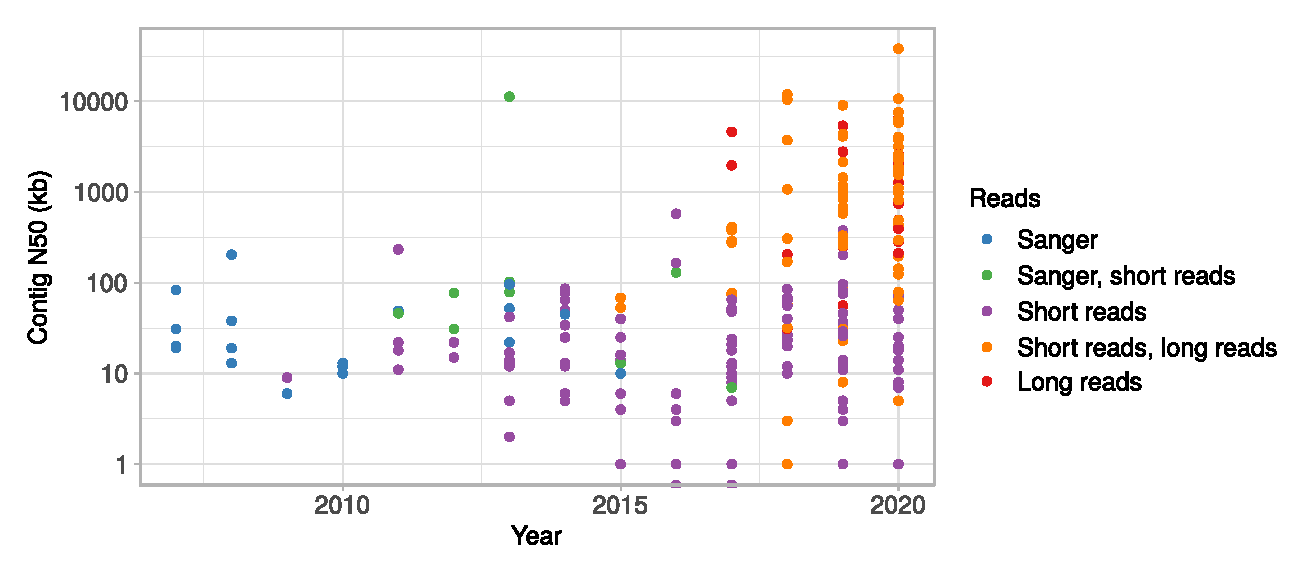
\includegraphics[width=\textwidth]{fig/review_contig_N50_year.eps}
    \caption{Contig N50 of non-vertebrate genome assemblies over time. The N50 represents the contiguity of an assembly and is defined as the length of the largest contig for which 50\% of the assembly size is contained in contigs of equal or greater length.}
    \label{fig:contig_N50_year}
\end{figure}

Third-generation sequencing has brought a whole new range of sequencing data, with the sequencing of long DNA molecules extending up to hundreds of thousands of bases \cite{pollard2018}. The two main players in the field, Pacific Biosciences (PacBio) and Oxford Nanopore Technologies (Nanopore), use two different kinds of technologies. PacBio developed Single Molecule Real-Time (SMRT) sequencing, where a complementary strand of DNA is produced from a single strand by addition of fluorescently labeled nucleotides. The fluorescent tag is released and the luminescence is interpreted as a base \cite{pacbio_smrt}. The resulting reads have a length around twenty kilobases (kb) and a high error rate, an issue recently addressed by the introduction of an extra step called Circular Consensus Sequencing (CCS). In CCS, the DNA polymerase passes multiple times on the same base on a circularized strand to produce High Fidelity (HiFi) reads that can achieve accuracy over 99\% \cite{pacbio_ccs}. \\

Nanopore sequencing uses a membrane with protein pores, through which an electrical current is flowing. DNA strands are pulled through the pores, with each passing nucleotide generating a distinct disruption signature in the current that can be inferred as a specific base \cite{nanopore}. The firm has specifically oriented its strategy toward a "do it yourself" approach, enabling sequencing in any lab and even directly in the field via a small portable device \cite{minion}. Researchers can control how they generate their sequencing data, contribute to protocol development, and develop their own basecalling \cite{basecallers} to increase the yield and improve the quality and length of the reads. Although Nanopore reads still exhibit a high error rate, their length keeps increasing to attain hundreds of kilobases to 1 Mb \cite{Jain2018}. Besides, the error rate has also been decreasing with the release of the new flow cells and the development of more accurate basecallers such as Bonito \cite{bonito}. \\

Long reads are now routinely included in genome assembly projects and have lead to N50 lengths much larger than short-read only assemblies (Figure \ref{fig:contig_N50_year}). A current limitation lies in the amount of DNA required to prepare long-read libraries. Still, long-read sequencing remains inaccessible for certain species: whereas Illumina sequencing can handle small DNA amounts, with a poor quality, long-read protocols require high-molecular weight DNA \cite{dna-extraction}. PacBio and Nanopore sequencing remain difficult when one animal is too small to provide a sufficient amount of DNA, especially when the organism requires extraction protocols that lead to overly fragmented DNA (for example, with coral skeletons). In addition, secondary metabolites associated to DNA molecules, or branched DNA structures, can also disturb the sequencing reaction. \\

\section{Genome assembly}

A variety of programs have been developed to assemble sequencing reads \textit{de novo}, taking advantage of different sequencing technologies while considering their limitations. Genome assembly aims to correctly reconstruct the original chromosome sequences from short or long, and accurate or error-prone fragments. Assemblers are typically based on one of the following paradigms: greedy, Overlap-Layout-Consensus, de Bruijn graphs. \\

\begin{table}
\caption{Sequencing approaches and associated assemblers.}
\centering
\begin{tabular}{|l|l|l|l|l|}
    \hline
    \textbf{Sequencing} & \textbf{Length} & \textbf{Accuracy} & \textbf{Methods} & \textbf{Assemblers}\\
    \hline
    First & 1 kb & High & Sanger & ARACHNE \cite{arachne}, Atlas \cite{atlas}, CAP3 \cite{cap3}, \\
    generation &  &  &  & Celera \cite{celera}, Euler \cite{euler}, JAZZ \cite{jazz},  \\
        &  &  &  & Minimus \cite{minimus}, MIRA \cite{mira}, phrap \cite{phrap}, \\
        &  &  &  & Phusion \cite{phusion}, SUTTA \cite{sutta}, TIGR \cite{tigr} \\
    \hline
    Second & 25-300 bp & High & 454, IonTorrent, & ABySS \cite{abyss,abyss2}, ALLPATHS \cite{allpaths}, \\
    generation &  &  & Solexa, SOLiD & CABOG \cite{cabog}, Edena \cite{edena}, Euler-SR \cite{euler-sr}, \\
        &  &  &  & Gossamer \cite{gossamer}, IDBA \cite{idba}, \\
        &  &  &  & JR-Assembler \cite{jr-assembler}, Meraculous \cite{meraculous}, \\
        &  &  &  & MIRA \cite{mira}, Newbler, NOVOPlasty \cite{novoplasty},  \\ 
        &  &  &  & PCAP \cite{pcap}, PERGA \cite{perga}, Platanus \cite{platanus},  \\
        &  &  &  & QSRA \cite{qsra}, Ray \cite{ray}, Readjoiner \cite{readjoiner}, \\
        &  &  &  & SGA \cite{sga}, SOAPdenovo \cite{soapdenovo}, \\
        &  &  &  & SOAPdenovo2 \cite{soapdenovo2} SPAdes \cite{spades}, \\
        &  &  &  & SSAKE \cite{ssake}, SUTTA \cite{sutta}, Taipan \cite{taipan}, \\
        &  &  &  & VCAKE \cite{vcake}, Velvet \cite{velvet} \\
    \hline
    Third & 10-100.000+ kb & Low & PacBio CLR, & Canu \cite{canu}, FALCON \cite{falcon-unzip}, Flye \cite{flye}, \\
    generation &  &  & Nanopore & HINGE \cite{hinge}, MECAT \cite{mecat}, \\
        &  &  &  & MECAT2 \cite{mecat}, miniasm \cite{miniasm}, \\
        &  &  &  & NECAT \cite{necat},NextDenovo \cite{nextdenovo}, \\
        &  &  &  & Ra \cite{ra}, Raven \cite{raven}, Shasta \cite{shasta}, \\
        &  &  &  & SMARTdenovo \cite{smartdenovo}, wtdbg \cite{wtdbg}, \\
        &  &  &  & wtdbg2 \cite{wtdbg2} \\
        & 20 kb & High & PacBio HiFi & Flye \cite{flye}, HiCanu \cite{hicanu}, hifiasm \cite{hifiasm}, \\ 
        &  &  &  & IPA \cite{IPA}, MIRA \cite{mira}, Peregrine \cite{peregrine}\\
    \hline
\end{tabular}
\label{tab:sequencing}
\end{table}


The assembly problem can be represented as a linear puzzle where the pieces are the reads. Reads match together when they have overlapping sequences. This puzzle could be intuitively solved by iteratively putting overlapping pieces together with the best matching piece: this greedy approach is an efficient heuristic to find the shortest common superstring of the set of reads (i.e., the shortest sequence that includes all the reads as substrings) \cite{greedy}. Greedy algorithms have been implemented for first-generation sequencing reads, for instance in TIGR \cite{tigr}, and were further applied in short-read assemblers like PERGA \cite{perga}, SSAKE \cite{ssake} and VCAKE \cite{vcake}. However, they cannot resolve complex, repetitive genomes: for this reason, greedy assemblers are mostly used nowadays to assemble small organelle genomes such as chloroplasts and mitochondria \cite{novoplasty}. \\

The Overlap-Layout-Consensus (OLC) paradigm was first described in 1979 by Rodger Staden \cite{olc} and is based on an overlap graph (Figure \ref{fig:olc}). The Overlap step consists in finding all the overlaps between all the reads and building a directed graph, where the nodes are the reads and the edges represent the overlaps between them. The Layout step removes redundant edges that can be inferred from other edges. Finally, the Consensus step finds an optimal path in the graph. The OLC paradigm has thrived with the program Celera \cite{celera}, which was used to assemble a human genome from a Sanger shotgun dataset \cite{venter2001}. \\

\begin{figure}
    \centering
    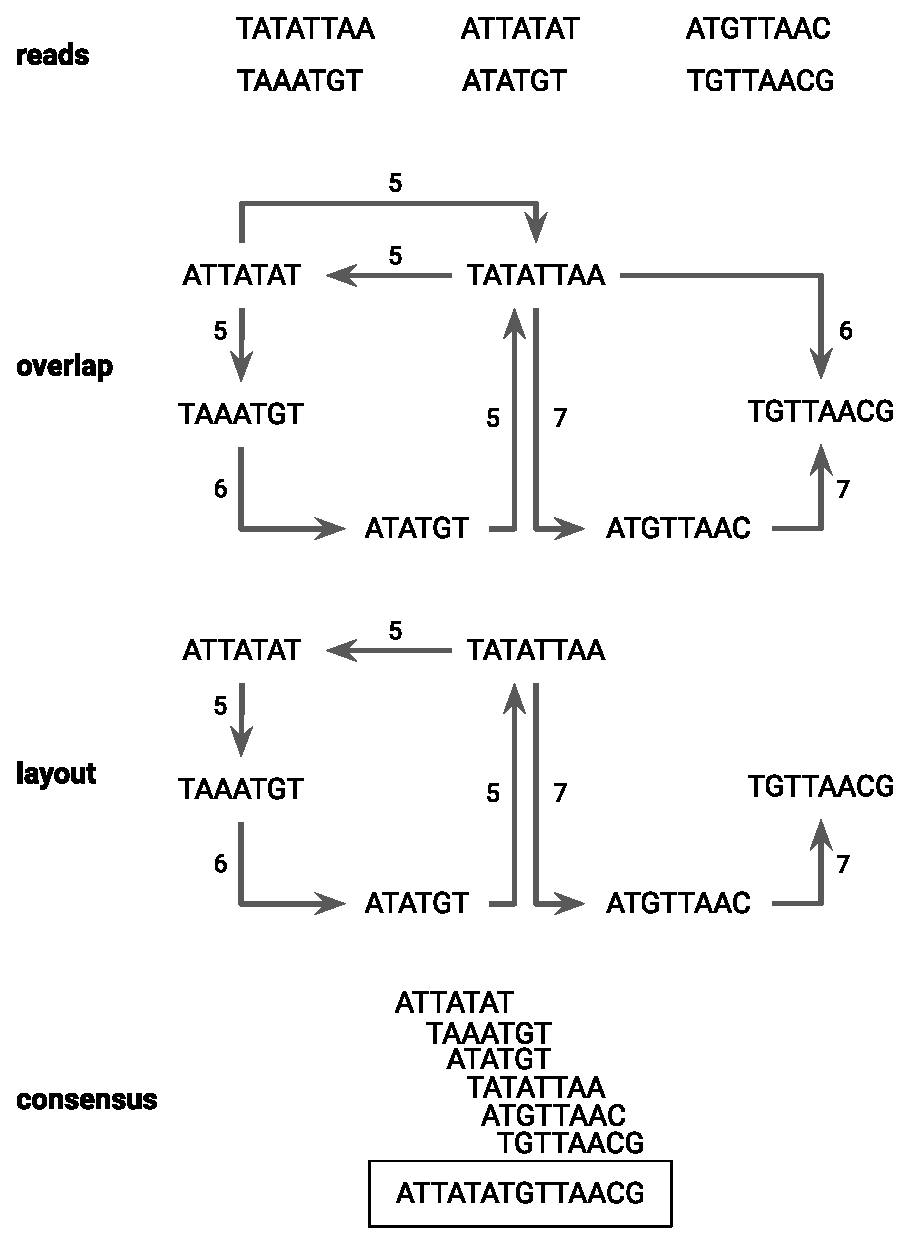
\includegraphics[width=\textwidth]{fig/review_olc.eps}
    \caption{Overview of Overlap Layout Consensus.}
    \label{fig:olc}
\end{figure}

De Bruijn Graphs (DBGs) (Figure \ref{fig:dbg}) are a well studied structure in graph theory, described by Nicolaas Govert de Bruijn in 1946 \cite{dbg} and before him by Camille Flye Sainte-Marie \cite{flyesaintemarie}. DBG-based assemblers require highly accurate reads in which errors are only substitutions, with no indels. They detect all the different sequences of a given \textit{k} length (\textit{k}-mers). Two \textit{k}-mers are connected in the graph when they have an overlap of a \textit{k}-1 length. The approach was first adapted for genome assembly of first-generation sequencing datasets \cite{Compeau2011} and was quickly implemented in multiple popular short-read assemblers, e.g. ABySS \cite{abyss, abyss2}, IDBA \cite{idba}, SOAPdenovo \cite{soapdenovo} and SOAPdenovo2 \cite{soapdenovo2}, SPAdes \cite{spades}, Velvet \cite{velvet}. \\

\begin{figure}
    \centering
    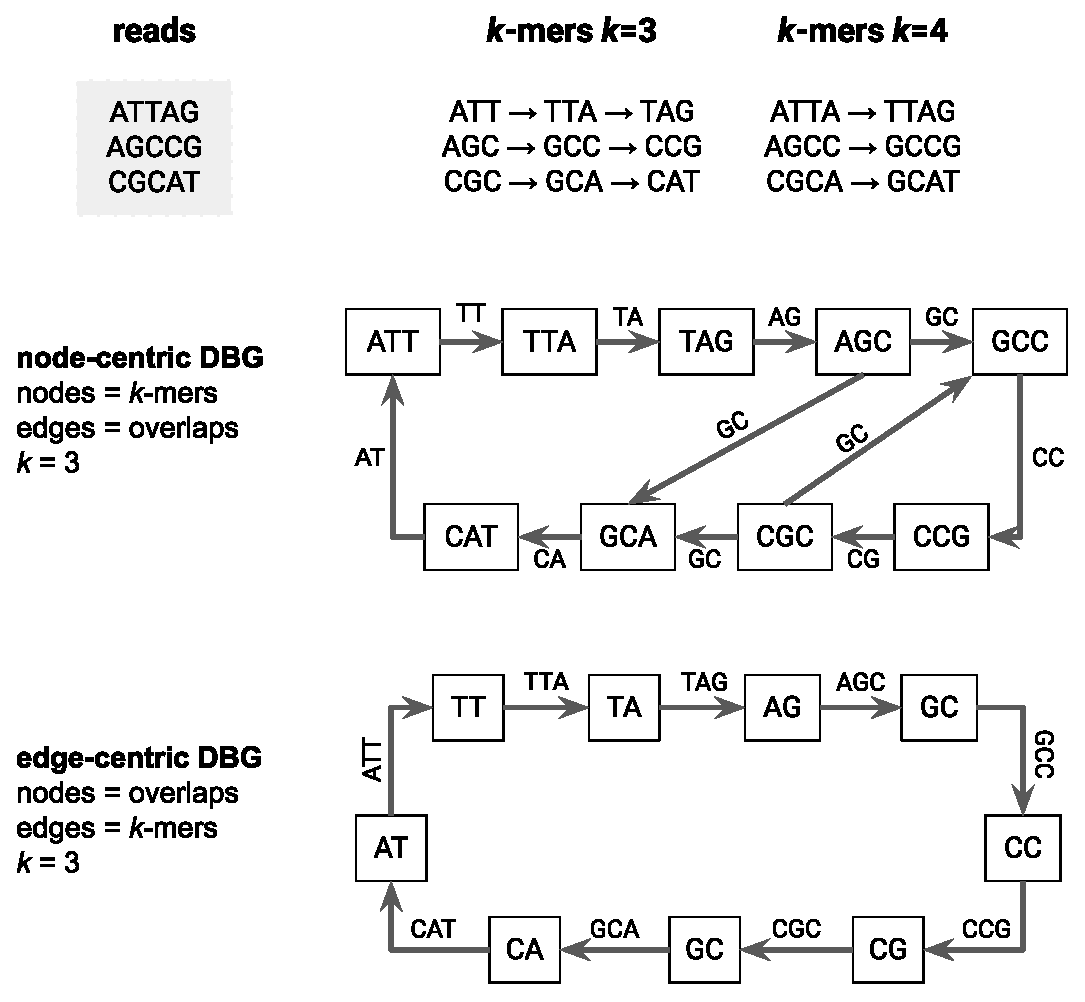
\includegraphics[width=\textwidth]{fig/review_de_bruijn_graph.eps}
    \caption{Overview of de Bruijn graphs.}
    \label{fig:dbg}
\end{figure}

With the advent of third-generation sequencing, OLC assemblers have benefited from a renewed interest whereas DBG-based ones are unsuited for long, low-accuracy reads, containing many erroneous \textit{k}-mers. Numerous assemblers have implemented OLC to produce \textit{de novo} assemblies from error-prone long-read datasets: Flye \cite{flye}, Ra \cite{ra}, Raven \cite{raven}, Shasta \cite{shasta}, wtdbg2 \cite{wtdbg2}. Now that HiFi reads bring a new type of high accuracy long reads, assemblers have been adapted to better handle these sequences, such as Flye (with adapted parameters), HiCanu \cite{hicanu} and hifiasm \cite{hifiasm}, and we can expect the development of new DBG assemblers adapted for large \textit{k}-mer values \cite{bankevich2020}. \\

From sequencing reads, assemblers build contiguous sequences called contigs. A perfectly assembled genome should have one contig representing each chromosome, but this is rarely achieved for eukaryotes. Assemblers need to find unambiguous paths in the assembly graph to reconstitute the chromosomes, but they often fail to do so due to the genomic structure: size, heterozygosity, repetitive content. Large genomes require a high amount of sequencing data in order to reach a sufficient depth to represent every loci. Genome sizes have a high variability (Figure \ref{fig:sizes}): in the phylum Cnidaria, some myxozoans have a genome size of only some tens of Megabases (Mb) (\textit{Kudoa iwatai}: 22.5 Mb, \textit{Myxobolus squamalis}: 53.1 Mb, \textit{Henneguya salminicola}: 60.0 Mb \cite{henneguya_salminicola}), while the hydrozoan \textit{Hydra oligactis} (1.3 Gigabases (Gb)) \cite{hydra_oligactis} has a genome size two orders of magnitude larger. Heterozygous regions constitute a major cause for breaks in assemblies of non-model animal genomes, as they generally have higher levels of heterozygosity than model species \cite{Leffler2012a}. Most assemblers try to build a haploid representation of all genomes, even for multiploid (i.e. diploid or polyploid) genomes. To this end, heterozygous regions are collapsed in order to keep a single sequence for every region in the genome. In an assembly graph, these heterozygous regions will manifest themselves as bubbles, where one contig (a homozygous region) can be connected to several other contigs (the alternative haplotypes of a heterozygous region). When the assembler is unable to select one path, the homozygous region is not joined with any of the haplotypes, leading to a break in the assembly. 

\begin{figure}
    \centering
    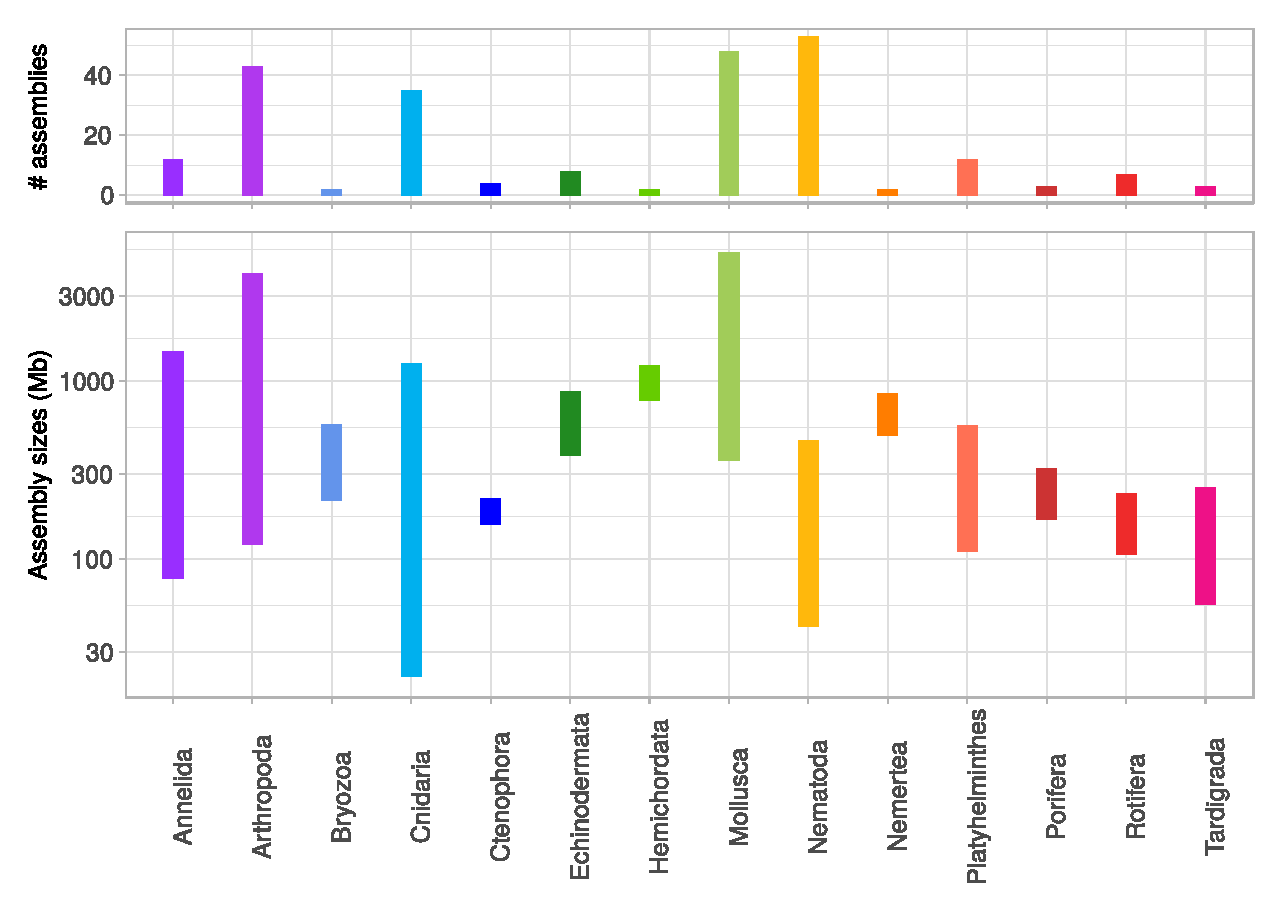
\includegraphics[width=\textwidth]{fig/review_assembly_sizes.eps}
    \caption{Assembly sizes. The top graph shows the number of assemblies included for each phylum and the lower part the corresponding assembly-size ranges.}
    \label{fig:sizes}
\end{figure}

\section{Assembly pre and post-processing}

\begin{table}
\caption{Assembly pre and post-processing tools for haploid assemblies.}
\begin{tabular}{|l|l|l|}
\hline
\textbf{Step} & \textbf{Sequencing data} &\textbf{Tools} \\
\hline
Reads filtering & Long reads & Filtlong \cite{filtlong} \\
\hline
Long reads & Short reads & CoLoRMAP \cite{colormap}, Hercules \cite{hercules}, Jabba \cite{jabba}, LoRDEC \cite{lordec}, \\
error correction &  & LoRMA \cite{lorma}, proovread \cite{proovread} \\
    \cline{2-3}
    & Long reads & Canu \cite{canu}, CONSENT \cite{consent}, Daccord \cite{daccord}, FLAS \cite{flas}, \\
    &  & NextDenovo \cite{nextdenovo}, MECAT \cite{mecat}, MECAT2 \cite{mecat}, NECAT \cite{necat} \\
\hline
Polishing & Short reads & ntEdit \cite{ntedit}, Pilon \cite{pilon}, POLCA \cite{polca} \\
    \cline{2-3}
    & Short \& long reads & Apollo \cite{apollo}, HyPo \cite{hypo}, Racon \cite{racon} \\
    \cline{2-3}
    & Long reads & Arrow \cite{quiver_arrow}, CONSENT \cite{consent}, Medaka \cite{medaka}, NextPolish \cite{nextpolish}, \\
    &  & Nanopolish \cite{nanopolish}, Quiver \cite{quiver_arrow} \\
\hline
Haplotigs purging & Long reads & HaploMerger2 \cite{haplomerger2}, purge\_dups \cite{purge_dups}, Purge Haplotigs \cite{purge_haplotigs} \\
\hline
Scaffolding & Short reads & Bambus \cite{bambus}, BATISCAF \cite{batiscaf}, BESST \cite{besst}, BOSS \cite{boss}, \\
    & Mate pairs & GRASS \cite{grass}, MIP \cite{mip}, Opera \cite{opera}, ScaffMatch \cite{scaffmatch}, \\
    &  & ScaffoldScaffolder \cite{scaffoldscaffolder}, SCARPA \cite{scarpa}, SCOP \cite{scop}, SLIQ \cite{sliq}, \\
    &  & SOPRA \cite{sopra}, SSPACE \cite{sspace}, WiseScaffolder \cite{wisescaffolder} \\
    \cline{2-3}
    & Long reads & LINKS \cite{links}, LRScaf \cite{lrscaf}, npScarf \cite{npScarf}, PBJelly \cite{pbjelly}, \\
    &  & RAILS \cite{rails}, SLR \cite{slr}, SMIS \cite{smis}, SMSC \cite{smsc}, \\
    &  & SSPACE-LongRead \cite{sspace-longread} \\
    \cline{2-3}
    & Genetic maps & ALLMAPS \cite{allmaps} \\
    \cline{2-3}
    & Optical maps & AGORA \cite{agora}, BiSCoT \cite{biscot}, OMGS \cite{omgs}, SewingMachine \cite{sewingmachine}, \\
    &  & SOMA \cite{soma} \\
    \cline{2-3}
    & Linked reads & ARBitR \cite{arbitr}, Architect \cite{architect}, ARCS \cite{arcs}, ARKS \cite{arks}, \\ 
    &  & fragScaff \cite{fragscaff}, Scaff10X \cite{scaff10X} \\
    \cline{2-3}
    & 3C/Hi-C & 3D-DNA \cite{3d-dna}, dnaTri \cite{dnatri}, GRAAL \cite{graal}, HiCAssembler \cite{hicassembler} \\
    &  & instaGRAAL \cite{instagraal}, Lachesis \cite{lachesis}, SALSA \cite{salsa}, SALSA2 \cite{salsa2} \\
\hline
Gap filling & Short reads & GapFiller \cite{gapfiller}, GAPPadder \cite{gappadder}, Sealer \cite{sealer} \\
    \cline{2-3}
    & Long reads & Cobbler \cite{rails}, FGAP \cite{fgap}, GMcloser \cite{gmcloser}, LR\_Gapcloser \cite{lrgapcloser}, \\
    &  & PBJelly \cite{pbjelly}, PGcloser \cite{pgcloser}, TGS-GapCloser \cite{tgsgapcloser} \\
\hline
\end{tabular}
\label{tab:scaffolding}
\end{table}

As obtaining high-quality chromosome-level contigs still remains challenging, upstream and downstream tools have been developed in conjunction with assemblers (Table \ref{tab:scaffolding}). Researchers can test numerous combinations of these tools to devise the pipeline that will yield the best assembly. \\

Long reads have the advantage over short reads that they result in more contiguous assemblies. Nevertheless, assemblies of PacBio Continuous Long Reads (CLR) or Nanopore reads can have remaining errors due to their low accuracy; while errors in PacBio CLR are random and are compensated with a high coverage, Nanopore reads have systematic errors in homopolymeric regions. Assemblies of error-prone long reads often necessitate additional processes to increase the quality. There are two possible strategies: correct the long reads prior to assembly, and polish the contigs after assembly. Correcting long reads can be done using only the long reads or by adding high-accuracy short reads. Many tools have been developed for both scenarii and have been thoroughly reviewed on multiple datasets \cite{correction_benchmark}. When tested on \textit{Caenorhabditis elegans} Nanopore reads, the error rate decreased from 28.93\% to less than 1\% (using Canu \cite{canu}, CONSENT \cite{consent}, FLAS \cite{flas}, Jabba \cite{jabba}, LORMA \cite{lorma} or MECAT \cite{mecat}). Some assemblers include a self-correction step in their pipeline, namely Canu \cite{canu}, MECAT \cite{mecat}, NECAT \cite{necat}, NextDenovo \cite{nextdenovo}. Assembling corrected reads is expected to yield contigs with higher quality and contiguity. Alternatively, or additionally, the contigs can be polished to reduce errors, using long reads and/or short reads. Polishing can be a more computationally efficient strategy: the reads are mapped solely to the draft assembly, while correction is usually based on an all-versus-all read mapping. \\

Assemblers are generally tested on model-organism datasets, and are ill-suited for non-model genomes with variable levels of heterozygosity. They often fail to collapse highly divergent haplotypes, causing artefactually duplicated regions that hinder subsequent analyses \cite{ko2021widespread}. Some long-read assemblers, Ra and wtdbg2, have been identified as less prone to retain uncollapsed haplotypes \cite{guiglielmoni2020}. Contigs can also be post-processed to remove these duplications with dedicated tools such as HaploMerger2 \cite{haplomerger2}, purge\_dups \cite{purge_dups} and Purge Haplotigs \cite{purge_haplotigs}. HaploMerger2 detects uncollapsed haplotypes based on sequence similarities, while purge\_dups and Purge Haplotigs also rely on coverage depth. \\

To improve the contiguity of an assembly, contigs can be grouped, ordered and oriented into scaffolds. These scaffolds may contain gaps, when the sequence that should connect two contigs cannot be retrieved, represented as a sequence of Ns, and these gaps can be reduced post-scaffolding with gap-filling tools. Chromosome-level scaffolds have become a standard in genome assembly publications: unlike fragmented assemblies, they can be used for synteny analysis, finding rearrangements, and to separate chromosomes from different species. Several sequencing techniques have been used to scaffold assemblies: mate pairs, long reads, genetic maps, optical mapping, linked reads, and proximity ligation \cite{ghurye2019modern}. Mate pairs are short reads with a large insert size (more than several kb), and have been widely used in next-generation assemblies. Among the 237 assemblies we surveyed, 78 included a mate-pair scaffolding step (Figure \ref{fig:hic}). Both genetic maps \cite{genetic_maps} and optical maps \cite{optical_maps} provide information on the linkage and relative position of a set of markers, spread over the genome, thus they can be used to anchor contigs. Genetic maps were used for the genome assemblies of the flatworm \textit{Schistosoma mansoni} \cite{schistosoma_mansoni2}, the copepod \textit{Tigriopus japonicus} \cite{tigriopus_japonicus} and the coral \textit{Acropora millepora} \cite{acropora_millepora2}. Although existing genetic maps provide precious resources, building one is particularly difficult as it requires breeding \cite{genetic_maps}, making it hardly accessible for wild species, and impossible for asexual species. Markers of optical maps are motifs in the sequence that are labeled and detected by a fluorescent signal. Companies such as Bionano or Nabsys propose this service to scaffold assemblies \cite{optical_scaffolding}, and this method was included in some non-vertebrate genome projects: several nematodes including \textit{Onchocerca volvulus} \cite{onchocerca_volvulus}, \textit{Ascaris suum} and \textit{Parascaris univalens} \cite{ascaris_suum2}, the tapeworms \textit{Echinococcus multilocularis} \cite{echinococcus_multilocularis} and \textit{Hymenolepis microstoma} \cite{hymenolepis_microstoma2}, and the chiton \textit{Acanthopleura granulata} \cite{acanthopleura_granulata}. \\

\begin{figure}
    \centering
    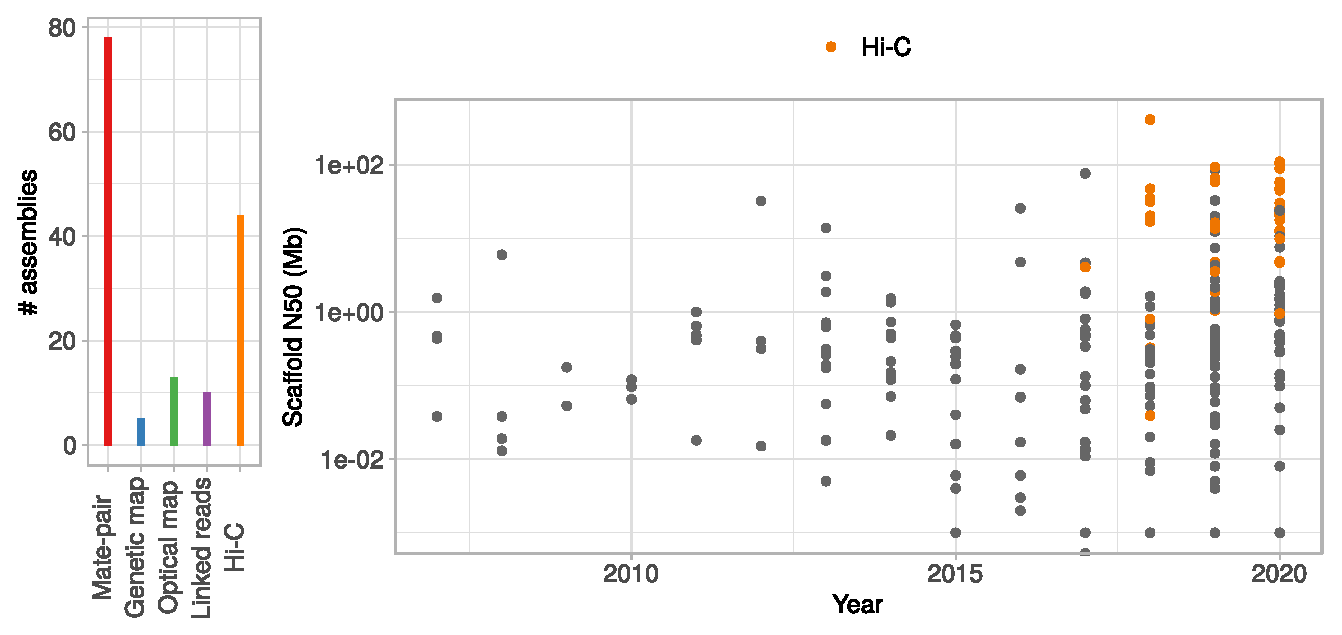
\includegraphics[width=\textwidth]{fig/review_scaffolding.eps}
    \caption{Assemblies scaffolding. Left: number of assemblies that included each scaffolding method. Right: scaffold N50 of non-vertebrate genome assemblies over time. The assemblies that included a Hi-C scaffolding step are highlighted in red; they form a cluster with a scaffold N50 over 1 Mb.}
    \label{fig:hic}
\end{figure}

Linked reads and proximity ligation are based on short-read sequencing, preceded by a specific library preparation. For linked reads, also called cloud reads, long fragments of DNA are barcoded and then sequenced. The company 10X Genomics was a leader of this technology, but they chose to discontinue its commercialization in June 2020. Linked reads have been used to scaffold the genomes of the coral \textit{Acropora millepora} \cite{acropora_millepora2} and the bee \textit{Lasioglossum albipes} \cite{lasioglossum_albipes}. As linked reads are also shotgun Illumina reads, these reads are sometimes used for assembly (using Architect \cite{architect} or Supernova \cite{supernova}) or polishing, as was done for the mosquito \textit{Anopheles funestus} \cite{anopheles_funestus}. \\

Proximity ligation techniques, based on capture of chromosome conformation \cite{Dekker2002}, were not originally developed with genome sequencing applications in mind. Instead, they aimed at investigating the interplay between chromosome 3D organization and DNA processes \cite{dekker2013exploring}. A popular genomic derivative of 3C, Hi-C \cite{Lieberman-Aiden2009} documents the average conformation of the genomes of a population of cells. Briefly, the approach consists in freezing the chromosome folding of each individual cell using chemical fixation by formaldehyde, which generates bonds between proteins and proteins, and proteins and DNA. Then, the genome is cut into fragments using a restriction enzymes, that are then ligated in dilute conditions. As a consequence, fragments that were trapped together by the crosslinking step are more prone to be ligated with each other, rather than with a fragment belonging to a different crosslinked complex. This results in chimeric fragments with respect to the original genome agencement, reflective of their 3D contacts \textit{in vivo}. The relative proportions of ligation events between all restriction fragments of a genome can then be quantified, in theory, through high-throughput sequencing. On average, and because of the polymer nature and physical properties of DNA, the frequency of contacts between a pair of loci reflects either their 1D \textit{cis} disposition along a chromosome, or their \textit{trans} disposition on two independent chromosomes \cite{flot2015contact, oddes2018}. Hi-C scaffolders have been developed following these principles: some follow a graph approach and use Hi-C links to join contigs (3D-DNA \cite{3d-dna}, SALSA2 \cite{salsa2}), whereas others exploit Markov Chain Monte Carlo (MCMC) sampling and Bayesian statistics to reorganize DNA segments into the scaffolds most likely to explain the observed interaction frequencies (GRAAL \cite{graal} and its later improved version instaGRAAL \cite{instagraal}). \\

The Hi-C protocol itself is becoming more and more accessible as commercial kits are now available (e.g. Arima Hi-C, Phase Genomics, or Dovetails Genomics). Besides, Dovetails Genomics uses both regular Hi-C and its own protocol for \textit{in vitro} proximity ligation, dubbed CHICAGO. Hi-C scaffolding proved efficient at bringing highly fragmented draft assemblies to chromosome-level scaffolds (Figure \ref{fig:hic}), and is now included in many genome projects for all sorts of non-vertebrates: the arthropods \textit{Varroa destructor} \cite{varroa_destructor} and \textit{Carcinoscorpius rotundicauda} \cite{carcinoscorpius_rotundicauda2}, the cnidarians \textit{Xenia sp.} \cite{xenia_sp} and \textit{Rhopilema esculentum} \cite{rhopilema_esculentum}, the echinoderms \textit{Lytechinus variegatus} \cite{lytechinus_variegatus} and \textit{Pisaster ochraceus} \cite{pisaster_ochraceus}, the molluscs \cite{scapharca_broughtonii} and \textit{Chrysomallon squamiferum} \cite{chrysomallon_squamiferum}, the nematods \textit{Caenorhabditis remanei} \cite{caenorhabditis_remanei2} and \textit{Heterodera glycines} \cite{heterodera_glycines2}, the platyhelminthe \textit{Schistosoma haemotabium} \cite{schistosoma_haematobium}, the poriferan \textit{Ephydatia muelleri} \cite{ephydatia_mulleri}, the rotifer \textit{Adineta vaga} \cite{adineta_vaga2}, the xenacoelomorph \textit{Hofstenia miamia} \cite{hofstenia_miamia}, and more. A compelling advantage of Hi-C scaffolding over other scaffolding methods is its ability to discriminate different organisms in a draft assembly: DNA from different organisms belong to distinct nuclei, thus they have no 3D interactions. This feature is especially useful for non-vertebrates with symbionts, that can hardly be eliminated from the host prior to sequencing, and are often targets for genome assembly as well. \\

\section{Assemblies evaluation}

A critical step in genome assembly is to estimate the quality of draft assemblies, and choose the best one for subsequent analysis. The first metric to assess is the assembly size and its adequacy with an estimated genome size. The size can be estimated experimentally with flow cytometry or Feulgen densitometry \cite{mulligan2014}, but these methods require a reference species for which the genome size is already well known, exposing them to errors induced by the reference genome size. Reference-free genome size estimation tools are typically \textit{k}-mer based approaches and use high-accuracy reads (e.g. Illumina, PacBio HiFi). These tools, such as BBtools \cite{bbtools}, GenomeScope \cite{genomescope} and KAT \cite{kat_evaluation}, build a \textit{k}-mer spectrum representing the number of \textit{k}-mers with a certain frequency of occurence. When the sequencing depth is sufficient, the \textit{k}-mer spectrum should display one or more peaks depending on the ploidy. For a haploid organism, there should be only one peak, whereas a diploid organism should have two peaks. The plot may also show a peak of \textit{k}-mers with a frequency of occurence close to zero, corresponding to erroneous \textit{k}-mers. Another recent tool called MGSE \cite{mgse} estimates genome size based on reads mapping to a highly continuous assembly of the same genome; this method can be used as a post-hoc analysis. \\

N50 is a popular metric that reflects the contiguity of an assembly: it is defined as the length of the largest contig for which 50\% of the assembly size is contained in contigs of equal or greater length. Some tools provide in addition the N75, N90, N99, computed in a similar fashion. The NG50 is a variant of N50 that refers to an estimated genome size instead of the assembly size. The target assembly can further be mapped against a reference assembly to detect misassemblies and break them: the N50 and NG50 of the resulting fragments are called NA50 and NGA50. All these metrics can be computed using QUAST \cite{quast}. For genome assemblies of non-model non-vertebrates, reference assemblies are seldom available, or they have a poor quality or contiguity that the new assembly aspires to improve. Therefore we will focus on reference-free evaluation methods. Table \ref{tab:assembly_stats} and Figure \ref{fig:evaluation} present an example of assembly evaluation for the recently published snail \textit{Achatina fulica} \cite{achatina_fulica} and coral \textit{Xenia sp.} \cite{xenia_sp}. \\

\begin{table}
\centering
\caption{Assembly evaluation of \textit{Achatina fulica} and \textit{Xenia sp.}.}
\begin{tabular}{|l|l|c|c|}
\hline
                &  & \textit{Achatina fulica} & \textit{Xenia sp.} \\
\hline
Basic statistics & Assembly size & 1.86 Gb & 222.7 Mb \\
                & N50 & 59.6 Mb & 14.8 Mb \\
                & N90 & 44.1 Mb & 6.9 Mb \\
                & Largest scaffold & 116.6 Mb & 22.5 Mb \\
                & Number of scaffolds & 1500 & 168 \\
                & Number of scaffolds larger than 1 Mb & 32 & 17 \\
                & N count & 3,600,500 & 194,000 \\
\hline
BUSCO completeness & Complete and single-copy BUSCOs & 84.4\% & 86.0\% \\
                & Complete and duplicated BUSCOs & 3.6\% & 2.2\% \\
                & Fragmented BUSCOs & 3.5\% & 3.5\% \\
                & Missing BUSCOs & 8.5\% & 8.3\% \\
\hline
Reads mapping & Short reads & 96.2\% & 87.8\% \\
                & Long reads & 81.62\% & 99.5\% \\
                & Hi-C & 70.2\% & 65.7\% \\
\hline
\end{tabular}
\label{tab:assembly_stats}
\end{table}

\begin{figure}
    \centering
    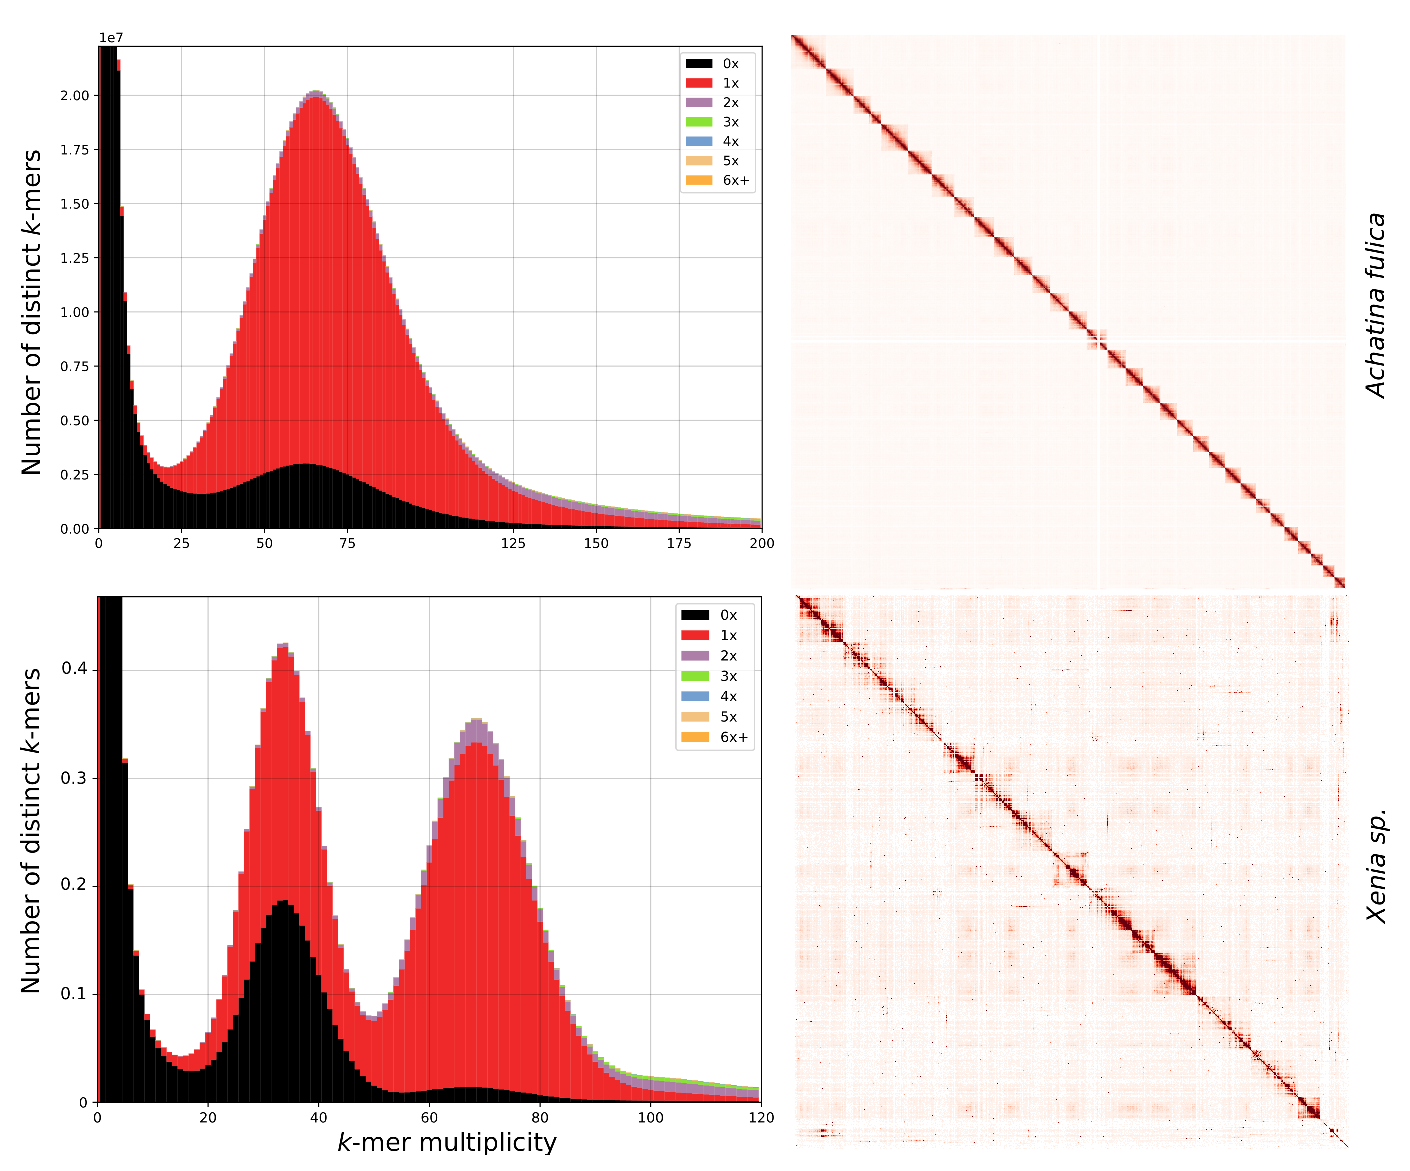
\includegraphics[width=\textwidth]{fig/review_assembly_evaluation.eps}
    \caption{Assembly evaluation of \textit{Achatina fulica} and \textit{Xenia sp.}. Left: KAT comparison of the \textit{k}-mers in the Illumina datasets v. the assembly. Right: Hi-C contact maps, with a binning of 300 for \textit{Achatina fulica}, 30 for \textit{Xenia sp.}.}
    \label{fig:evaluation}
\end{figure}

Another feature to optimize is the completeness of the genome, usually based on orthologs or \textit{k}-mers. BUSCO \cite{busco_evaluation} searches for orthologs in a user-provided lineage; the current Metazoa lineage (designated as Metazoa odb10) contains 954 features. Assemblies are evaluated based on the proportion of orthologs to these 954 genes that can be retrieved into them; yet, some features are systematically missing in some genomes as they are absent from these species. More specific lineages are available for arthropods, insects, vertebrates, mammals, as many assemblies are available for these groups, but other metazoan phyla suffer from their lack of resources. Consequently, BUSCO is most powerful when comparing several draft assemblies for one genome. BUSCO scores provide information on complete single-copy and duplicated features, and the latter can be used to detect improperly duplicated regions in a haploid assembly. However, BUSCO scores are limited to genomic regions and cannot report for non-coding ones. \\

\textit{k}-mer completeness scores do not present such limitations: KAT assesses the completeness of a whole assembly based on its representation of \textit{k}-mers from a high accuracy sequencing dataset. The \textit{k}-mer spectrum should display one or several peaks depending on the ploidy of the genome: one peak for a haploid genome; two peaks for a diploid genome, the first depicting heterozygous \textit{k}-mers, and the second for homozygous \textit{k}-mers. Depending on the ploidy of the genome, every \textit{k}-mers should be represented in the assembly as many times as they actually are in the genome. \\

Both \textit{Achatina fulica} and \textit{Xenia sp.} have high BUSCO scores (against the lineage Metazoa odb10), yet slightly below 90\%, and they have few duplicated BUSCO features. The \textit{k}-mer spectrum of \textit{Achatina fulica} only shows one peak around 70X (Figure \ref{fig:evaluation}, top left). These \textit{k}-mers are expected to be represented exactly once, which is the case for the majority; there are almost no \textit{k}-mers that appear twice in the assembly (in purple), but there is a noteworthy amount of missing \textit{k}-mers (in black). For \textit{Xenia sp.}, the \textit{k}-mer spectrum has two peaks with a \textit{k}-mer multiplicity around 35X and 70X (Figure \ref{fig:evaluation}, bottem left). The first peak, representing heterozygous \textit{k}-mers, shows that a portion is represented once in the assembly, while the rest is missing, as expected in a collapsed assembly. The second peak, for homozygous \textit{k}-mers has a majority of \textit{k}-mers represented once, and some \textit{k}-mers either absent or duplicated. These assemblies seem overall properly collapsed and complete. \\

KAD, for \textit{k}-mer abundance difference \cite{kad}, proposes an alternative \textit{k}-mer-based evaluation. This tool does not compute an overall completeness score, but instead classifies \textit{k}-mers based on their abundance in the assembly and the sequencing dataset: good \textit{k}-mers, erroneous \textit{k}-mers (absent from the dataset), overrepresented \textit{k}-mers (duplications), and underrepresented \textit{k}-mers (collapsed repetitions). \\

Assemblies need to be screened for contaminants, to tell apart the sequences coming from the target and from other species. Contaminants may originate from the environment, the symbiont, or be artificially introduced by the sequencing process. Blobtools \cite{blobtools} and BlobToolKit \cite{blobtoolkit} aim to identify them with GC content, coverage depth and taxonomy assignment using the NCBI TaxID. Discriminating bacteria in metazoan assemblies is usually straightforward based on their distinct GC percentage. The task is more challenging when the target metazoan genome is mixed with other eukaryotes or even metazoans, especially when these species are absent from databases. Chromosome-level assemblies reduce the risk of contamination, as downstream analysis can be run exclusively on sequences that were anchored to the main scaffold. In addition, with Hi-C data, sequences from different species can be separated based on their absence of \textit{trans} interactions. Contamination can lead to false conclusions: for instance, a study on a highly fragmented genome assembly (N50 = 16 kb) of the tardigrade \textit{Hypsibius dujardini} assumed that about 17\% of its genome derived from horizontal gene transfers \cite{hypsibius_dujardini1}, when these sequences were in fact contaminants \cite{hypsibius_dujardini2}. 

When Hi-C data are available, contact maps, i.e. the representation of the paired-end reads from the Hi-C library aligned on the resulting scaffold, procure another evaluation asset to search for misassemblies. The contact map is expected to show heightened frequencies for each chromosome, in a chromosome-level assembly, and these interaction frequencies should decrease with increased distances separating loci on the sequence, based on the distance law. For \textit{Achatina fulica}, 30 chromosome-level scaffolds (out of 31) display relatively consistent and regular contact patterns, representing well individualized entities in the contact map (Figure \ref{fig:evaluation}, top right). By contrast, the contact map of \textit{Xenia sp.} does not display such patterns, with multiple \textit{trans} contacts appearing between the scaffolds and most likely corresponding to scaffolding errors. \\

\section{Phasing assemblies}

As collapsing multiploid genomes can be difficult for highly divergent regions and frequently causes breaks in the assembly, an intuitive solution would be to phase genomes to retrieve all haplotypes. Phased assemblies represent a whole different challenge as they necessitate to correctly associate alleles, i.e. different versions of a heterozygous region \cite{unzipping}. A first approach, called trio-binning, is to assemble one individual using sequencing data from the individual itself and its parents \cite{triocanu}; yet this method is only adapted when the parents can be identified, and is inapplicable on asexual species. Some tools are able to reconstruct haplotypes from collapsed assemblies using long reads, namely HapCUT2 \cite{hapcut2} and WhatsHap \cite{whatshap}. Ideally, genomes should be uncollapsed, as can be done with Bwise \cite{bwise} and Platanus-Allee \cite{platanus-allee} using short reads and FALCON-Unzip \cite{falcon-unzip} using PacBio CLR or HiFi. FALCON-Unzip uses the output from the FALCON assembler, that includes both a haploid assembly and alternative haplotigs for heterozygous regions, to associate haplotypes based on long reads. Phased assemblies of low-accuracy long reads are limited, as small heterozygous regions were confused with errors; this led to haplotypes being erroneously collapsed. \\

HiFi reads have made a disruption in the fields of genomics: they are especially well-suited for phased assemblies thanks to their length and low error rate, and they have already been used to produce phased assemblies of a human \cite{phased_human} and the potato \textit{Solanum tuberosum} \cite{potato}. Nevertheless, sequencing HiFi reads can remain inaccessible for non-model organisms as pure DNA is necessary. \\

Many organisms have already been assembled using low-accuracy longs reads and high-accuracy short reads, thus an alternative is to correct long reads with short reads using a tool that conserves haplotypes such as Ratatosk \cite{ratatosk}. Phased long-read assemblies can be further polished with adequate programs (e.g. Hapo-G \cite{hapog}). As Hi-C has already demonstrated its efficiency to scaffold haploid assemblies, the principles were further exploited in ALLHiC \cite{allhic} and FALCON-Phase \cite{falcon-phase} to phase assemblies while increasing their contiguity: as alleles from one haplotype belong to one chromosome, these alleles have higher Hi-C interaction frequencies together than with alleles from alternative haplotypes. \\

Phasing-specific evaluation methods are still scarce, and publications of phased assembly rely on various datasets to prove their correctness (e.g. parental assemblies \cite{phased_human}). Merqury \cite{merqury} proposes a \textit{k}-mer-based approach, inspired by KAT, and computes plots and scores to assess phasing completeness and find haplotype switches. However, similarly to trio-binning, it requires parental data. \\

\section{Outline of the thesis}

This first chapter introduced the principles of DNA sequencing, genome assembly, and the difficulties specific to non-vertebrate animals. This thesis is divided into two main sections: Chapters 2, 3 and 4 describe methodologies and tools for genome assembly, whereas Chapters 5, 6 and 7 present the application of these methods to genome projects. \\
Chapter 1 evaluates the performances of seven long-read assemblers, and more specifically their behavior on non-model genomes with variable levels of heterozygosity, based on the example of the rotifer \textit{Adineta vaga}. The end goal of this study is to produce high-quality collapsed contigs from multiploid genomes. In Chapter 2, the strategy is the opposite, as the aim is to obtain uncollapsed, phased assemblies. This part presents the tool GraphUnzip, which takes advantage of assembly graphs, long reads and Hi-C reads to yield phased gap-less supercontigs with a high contiguity. Chapter 3 takes contigs to scaffolds with the Hi-C scaffolder instaGRAAL, a new version of GRAAL. Chapter 4, 5 and 6 describe the genome assemblies of \textit{Adineta vaga}, \textit{Astrangia poculata} and \textit{Flaccisagitta enflata}, using the strategies identified in Chapter 2 for long-read assembly, and instaGRAAL for Hi-C scaffolding.  \\